\chapter{Experiment Results}
\label{chapterlabel7}

\section{Experiment Setup, Dataset Introduction and Measurement Method}

In this part, the results of two experiments for Chapter 3 and 4 will be presented. At first, we will demonstrate that the performance of counting feature on non-linear regression model is comparable to that of one-hot binary feature of linear regression model. Secondly, we will show that counting feature performs significantly better than binary feature in cross-domain learning problem. 

The first experiments will be done on the dataset of Adform and iPinYou, the details of iPinYou dataset can be found in \cite{zhang2014real}, the details of Adform dataset can be seen in Table \ref{tab:triii}.

\begin{table}[h]
\begin{tabular}{l | c | p{5cm}}
Column Number & Description & Example\\
\hline \hline
1 & user country id & 208\\
2 & cookie id & qTXoig== \\
3 & log time & 2015-03-14 00:00:05\\
4 & log date id & 2015-03-14 \\
5 & log time hour & 0\\
6 & client ID & 1414\\
7 & placement ID & 1305663 \\
8 & inventory source ID & 31\\
9 & domain & +Ueytw== \\
10 & url & J6vrEw==;+Ueytw==;bxXScQ==\\
11 & position ID & 1\\
12 & size & 930x180\\
13 & browser ID & 226\\
14 & OS ID & 132\\
15 & user agent & a7fQug==;Ofd6Ig==\\
16 & screen size ID & 2057000011\\
17 & visited domains & 1508581;1768451;1768999\\
18 & visited logpoints & 1769969 \\
19 & clicker& 1 \\
\end{tabular}
\caption{Adform Dataset field description}
\label{tab:triii}
\end{table}

The data provided by Adform is valuable for our research. Adform is a media tech vendor for media agencies, advertisers, trading desks and publishers which offers the world’s only programmatic brand-led media platform supporting all aspects of multi-screen brand advertising. The company tech stack involves a demand side platform, third party ad server, data management platform, private marketplace, programmatic publisher ad server and a robust creative suite. 

By omitting the redundant and noisy information in the dataset, for the experiment of comparing the performance of counting feature and binary feature we choose 14 fields data to train our model, which are 
\begin{itemize}
\item User Information : We choose \textit{user country ID} which can show the region of the user, \textit{log date} and \textit{log time} to show user's behavior that when to go online, and \textit{visitied domains} and \textit{visited logpoints} which shows the user's history.
\item Advertisement Information : We choose \textit{clicker}, shows how many times this ads have been clicked, \textit{size}, \textit{position ID} to show the advertisement's basic information, \textit{client ID} shows the advertisers this ad belong to, representing the type of the ad, and \textit{placement ID} showing which campaign is the ad from, as well as \textit{inventory source ID} which involves the exchanger information
\item Context Information : We use  \textit{OS ID} and \textit{brower ID} show the device, OS and brower information of the user
\end{itemize}

The whole process of feature generation is in Figure \ref{fig:datalabel}, the data from 14 consecutive days are randomly divided into datasets of training, test and count dataset. Training and test datasets have obvious meaning, for count dataset, we use it to, first, building the feature index for binary feature, second, calculating the frequency and average CTR value of each item for counting features. The reason we do this is to make sure the counting feature values are independently generated from training or test dataset, so that overfitting can be avoided and the process for generating binary and counting features are the same to make sure fairness.

\begin{figure}[h]
\centering
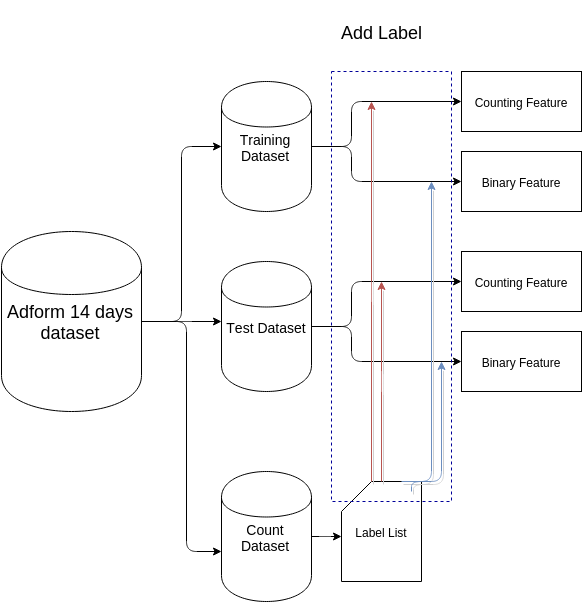
\includegraphics[width=\columnwidth]{datalabel.png}
\caption{Process of label counting feature and binary feature}
\label{fig:datalabel}
\end{figure}

And for the experiment of cross domain problem, we divide the datasets into different campaigns using \textit{client ID} and \textit{Placement ID}, we choose 12 rest of the fields to train the model.

The second experiment will be the usage of counting feature in \textit{Cross Domain problem}, we will do the experiment in the following scenario. An advertising company serves for different clients for CTR prediction. Based on the information from old campaigns, it hopes to get accurate CTR prediction result for new campaigns without training new model but directly make use the off-the-shelf model derived from old campaigns. 

In this experiment, the whole 14 days dataset will be split based on the client id so that in each sub dataset all impressions are from a unique client. To simulate the real world situation that the ad data is not static but performs as a continuous data stream, the new campaign dataset will be further divided into smaller data capsules. Then on the one side, the old campaign dataset will be transformed into binary feature dataset then the model will be trained based on it. Then capsules will be sent into the model in sequence to estimate its CTR thus AUC for test dataset will be obtained. 
While on the other side, counting feature bears the advantage that its number of features are limited, and feature values are continuous. So unlike 0-1 binary feature, it is possible to update the feature values as more information from new campaign arrives with fixed model weights. The representation of two scenarios can be represented as follows in Figure ~\ref{fig:binary}

\begin{figure}[t]
\centering
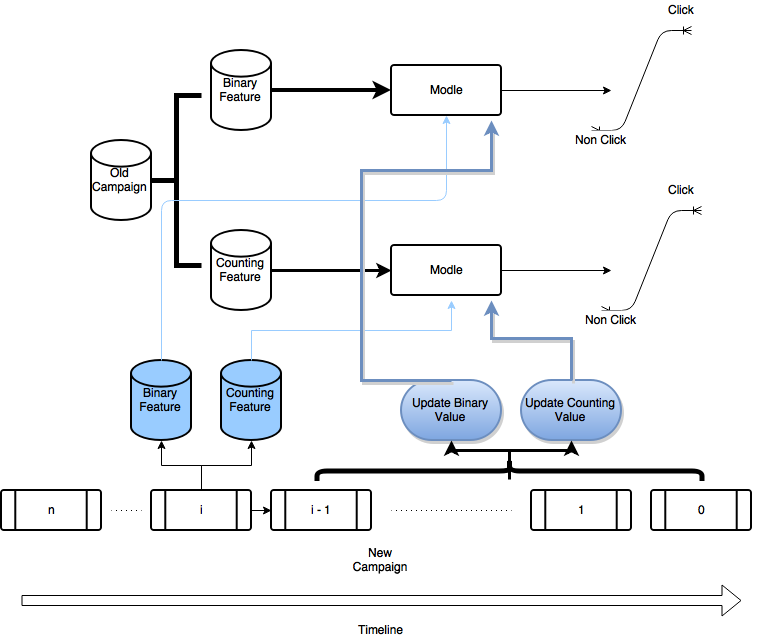
\includegraphics[width=\columnwidth]{countingdiagram.png}
\caption{Estimate new campaign CTR using Binary Feature and Counting Feature Comparison}
\label{fig:binary}
\end{figure}

\section{Performance Comparison of Binary and Counting Feature in CTR prediction Problem}

In this section two experiments are conducted to compare the CTR prediction performance of Binary and Counting feature in terms of logistic regression and gradient boosting regression tree (GBRT) model. The first experiment is based on the public dataset from iPinYou, which was released by the Chinese RTB company iPinYou for global RTB algorithm competition in 2013. The dataset includes logs of ad auctions, bids, impressions, and also clicks \cite{zhang2014real}. All the features except for \textit{Usertag} are used in the experiment due to the bias in that feature. 3 campaigns are selected to show the result, the result is as follows in Figure \ref{fig:ipinyou}:
\begin{figure}[h]
    \centering
    \begin{subfigure}[b]{0.3\textwidth}
        \centering
        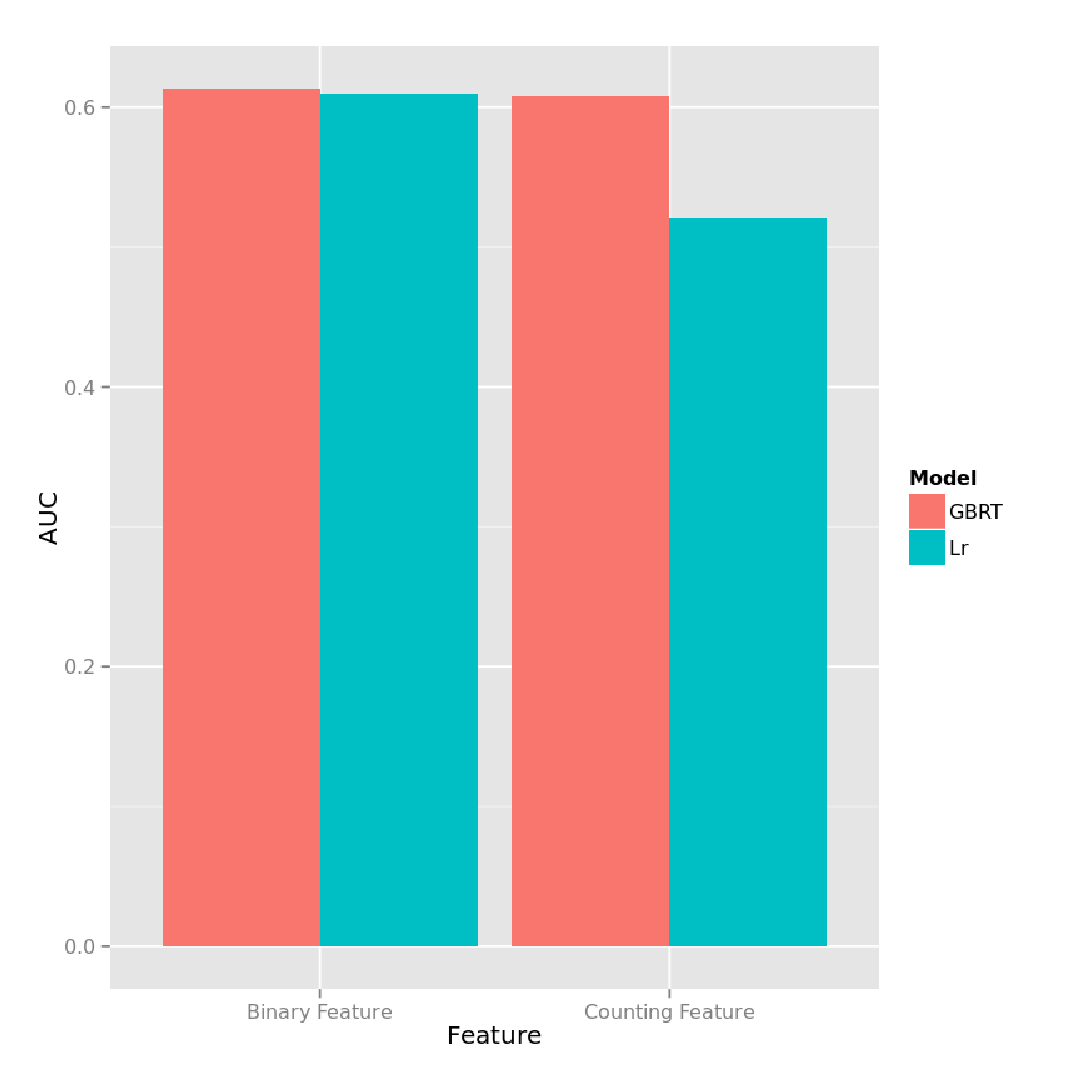
\includegraphics[width=\textwidth]{2261.eps}
        \caption{Performance of 2261}
        \label{fig:2261}
    \end{subfigure}
    \hfill
    \begin{subfigure}[b]{0.3\textwidth}
        \centering
        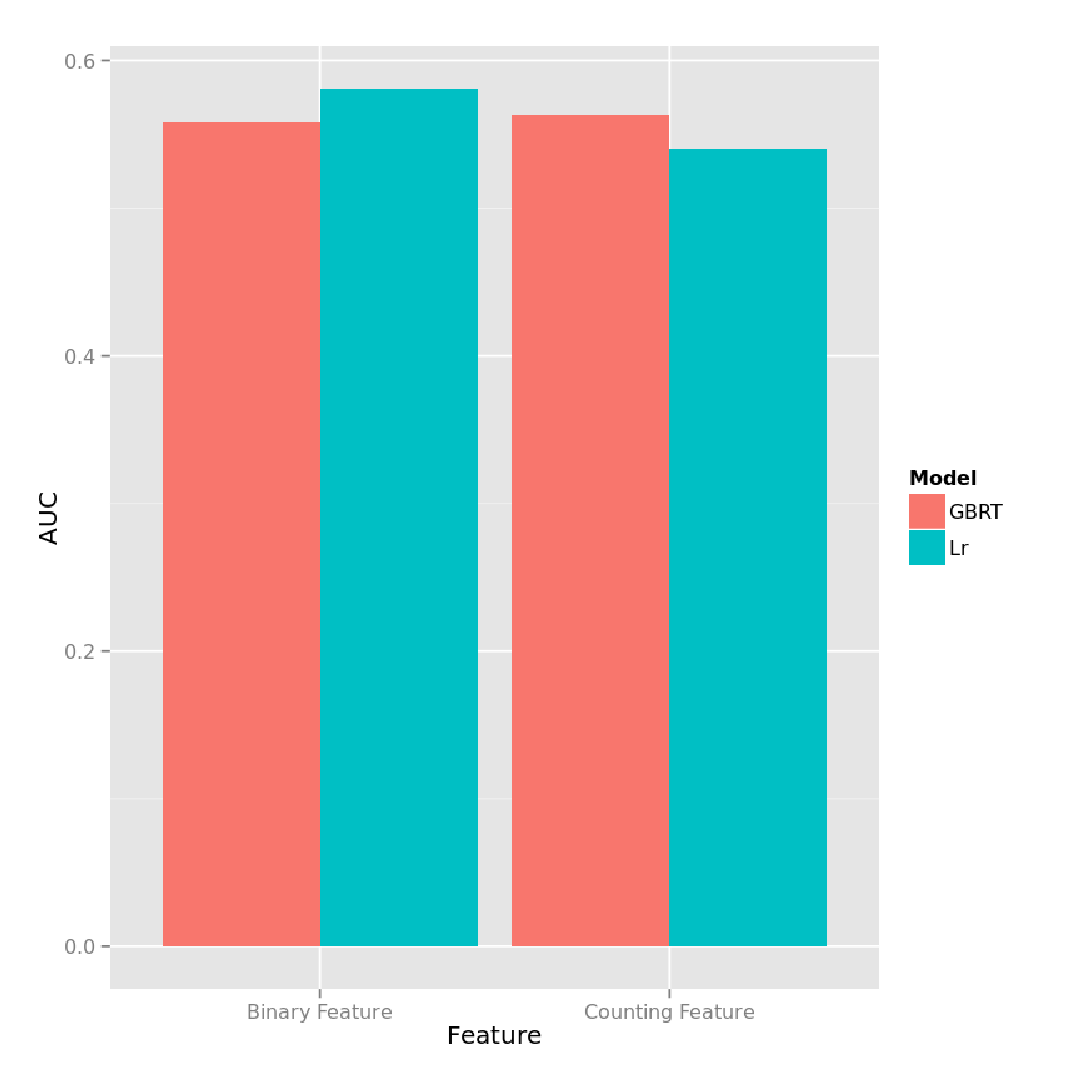
\includegraphics[width=\textwidth]{2997.eps}
        \caption{Performance of 2997}
        \label{fig:2997}
    \end{subfigure}
    \hfill
    \begin{subfigure}[b]{0.3\textwidth}
        \centering
        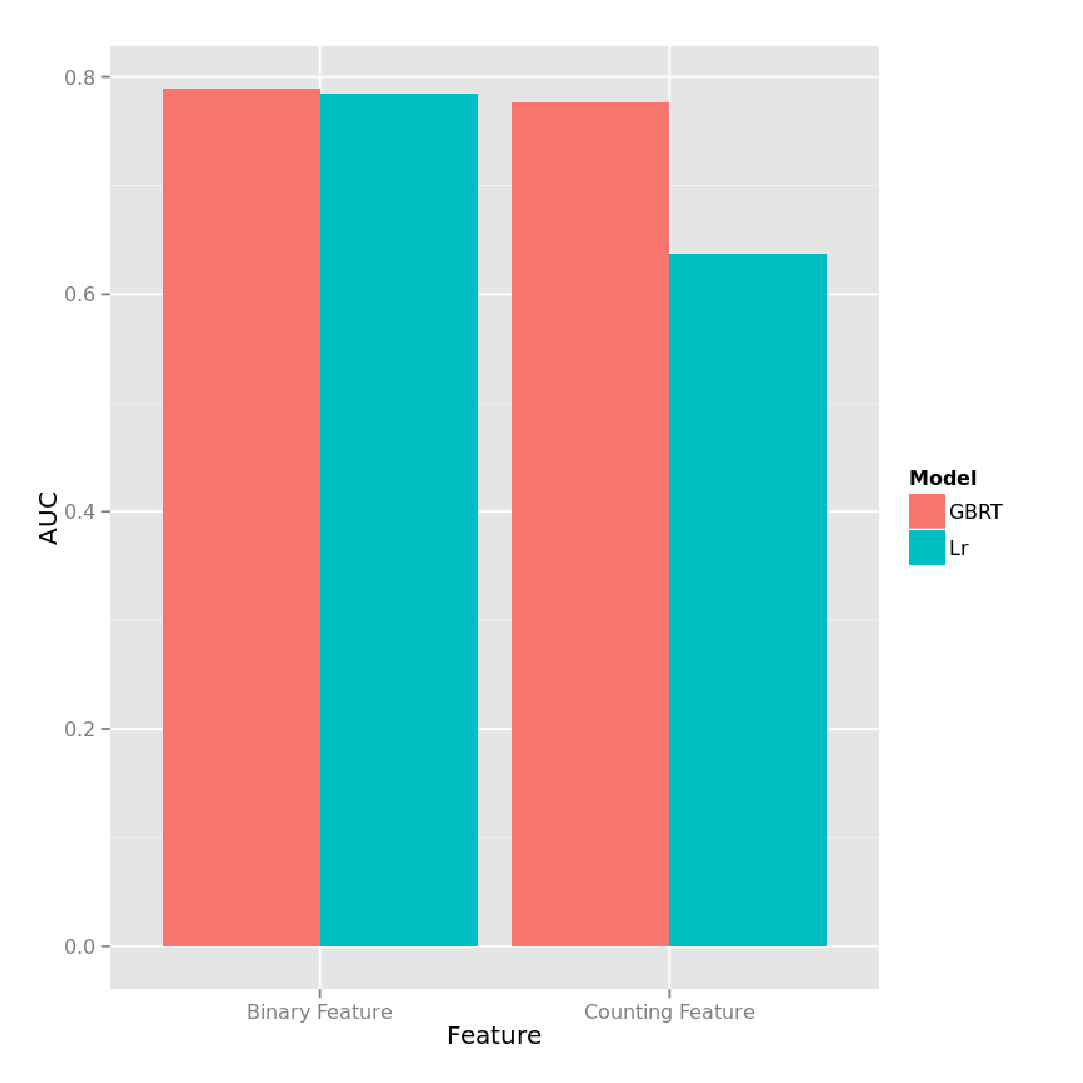
\includegraphics[width=\textwidth]{3386.eps}
        \caption{Performance of 3386}
        \label{fig:3386}
    \end{subfigure}
    \caption{Comparison of performance of counting feature and binary feature in terms of logistic regression model and GBDT model}
    \label{fig:ipinyou}
\end{figure}

For Adform dataset, we select the top 10 campaigns in terms of the number of impressions, and do the same experiment, the results can be seen in Table \ref{tab:adform} 


\begin{table}
\tiny
\centering
  \begin{tabular}{|c|c|c|c|c|c|c|c|c|}
    \hline
    \multirow{3}{*}{AdForm Data} &
      \multicolumn{4}{c}{Binary Feature} &
      \multicolumn{4}{c|}{Counting Feature}  \\ 
      & \multicolumn{2}{c|}{LR} &
      \multicolumn{2}{c|}{GBDT} &
      \multicolumn{2}{c|}{LR} &
      \multicolumn{2}{c|}{GBDT} \\
    & AUC & RMSE & AUC & RMSE & AUC & RMSE & AUC & RMSE \\
    \hline
    8908 & 0.80262456 & 0.09501891 & 0.888714 & 0.089650 & 0.72991575& 0.09666564 & 0.918956 & 0.084637\\
    \hline
    14501 & 0.89823655 & 0.07899161 & 0.936264 & 0.071931 & 0.87440427 & 0.08208775 & 0.952850 & 0.066130\\
    \hline
    22134 & 0.67120365 & 0.11098081 & 0.885912 & 0.106765 & 0.62599030 & 0.11258175 & 0.907666 & 0.103013\\
    \hline
    1414 & 0.72499931 & 0.17720046 & 0.857426 & 0.165498 & 0.67158281 & 0.18037752 & 0.880398 & 0.163203\\
    \hline
    20224 & 0.90021574 & 0.07469178 & 0.963710 & 0.069388 & 0.79591829 & 0.07517684 & 0.977535 & 0.065842\\
    \hline
    16280 & 0.87195981 & 0.04301431 & 0.951357 & 0.038806 & 0.81802916 & 0.04514749 & 0.885012 & 0.039111	\\
    \hline
    12482 & 0.80125347 & 0.04842428 & 0.923162 & 0.046272 & 0.76619990 & 0.04970136 & 0.951100& 0.044128\\
    \hline
    1371 & 0.79818709 & 0.09283530 & 0.899852 & 0.084791 & 0.79291810 & 0.10990528 & 0.942543 & 0.081489\\
    \hline
    15140 & 0.85500486 & 0.06924050 & 0.939948 & 0.066548 & 0.77392638 & 0.07250272 & 0.905959 & 0.066633\\
    \hline
    20762 & 0.64999602 & 0.02021880 & 0.858127 & 0.020300 & 0.85541771 & 0.01706115 & 0.941716 & 0.019269\\
    \hline
  \end{tabular}
  \caption{Performance comparison of counting feature and binary feature in terms of logistic regression and GBDT for adform dataset}
 \label{tab:adform}
\end{table}

For the whole dataset of 14 days, the result is in Figure \ref{fig:adform}

\begin{figure}[h]
\centering
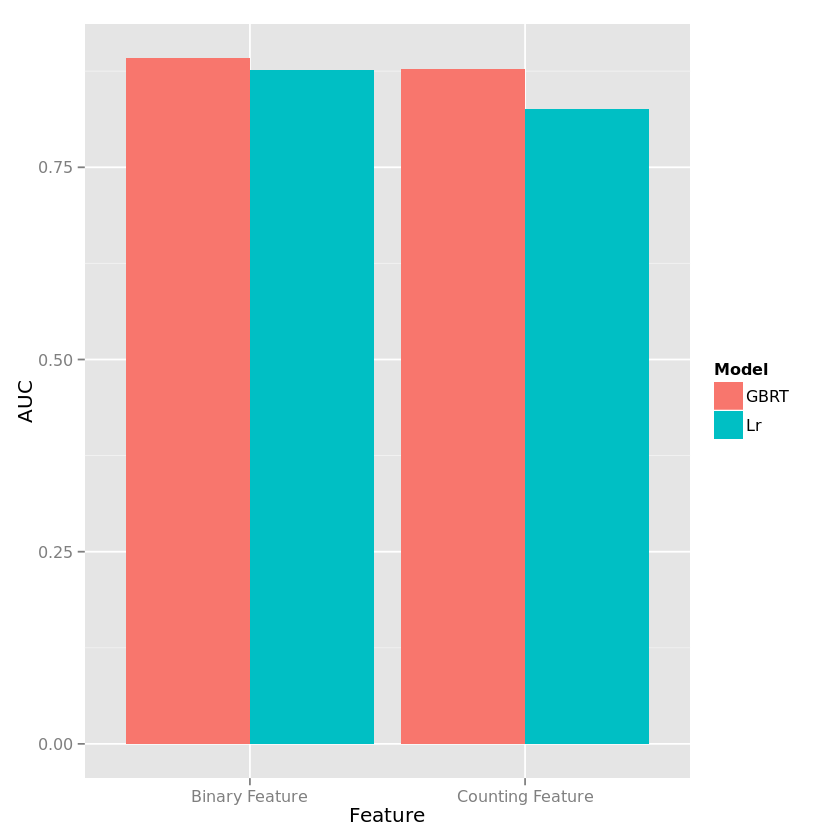
\includegraphics[width=\columnwidth]{adform.png}
\caption{Performance of counting feature and binary feature of logistic regression model and GBDT for Adform dataset}
\label{fig:adform}
\end{figure}

From the above result we can say that counting feature can obtain comparable or even better performance in CTR prediction than binary feature when using non-linear model.


\section{Performance Comparison of Binary and Counting Feature in Cold Start Problem}



\begin{figure}[h]
\centering
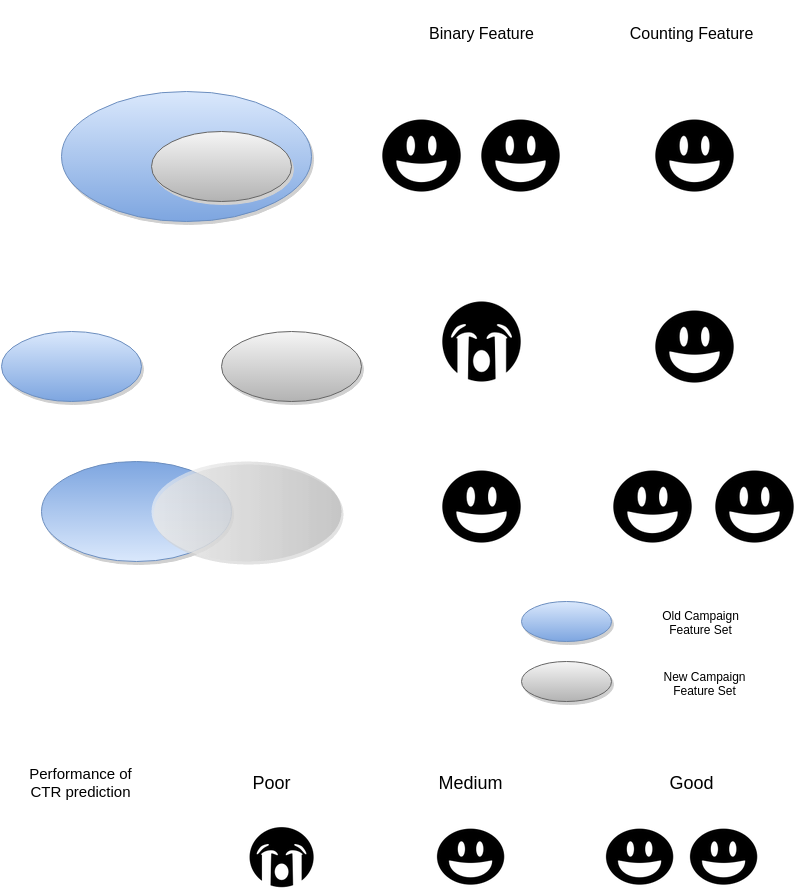
\includegraphics[width=\columnwidth]{bias.png}
\caption{Three types of relation of feature sets between train dataset and test dataset}
\label{fig:datasetbias}
\end{figure}

In this part, the experiments will be done based on the dataset provided by a ad company in March which includes the data for 14 consecutive days, the dataset are separated by client id so that in each small dataset there are only the impressions from one unique client. In this experiment, the client with more than 500,000 impression are chosen so that 10 sub datasets are obtained which are from distinct clients. 


\iffalse
\begin{table}[t]
 \centering
 \begin{tabular}{ ||c c || } 
 \hline
 Client id  & Number \\
 \hline
 20762 & 1068606 \\ 
  15140 & 764355 \\ 
   1371 & 576709 \\ 
   12482 & 557120\\
 \hline
 \end{tabular}
 \caption{Four Biggest clients}
 \label{tab:campainid}
 \end{table}
 
\fi

The Figure \ref{fig:datasetbias} above shows the truth that dataset significantly decide upper bound of the accuracy to predict CTR. above performance comparison of binary feature and counting feature on CTR estimation reveals that performance of counting feature using non-linear regression model is comparable to that of binary feature using linear regression model, the precondition is that the training and test dataset share most of the features. However, in real world we will always be faced up with the situation that the information is unbalanced in train and test dataset. We define \textit{Feature Set} as a criterion to measure the information obtained in the dataset, which is represented by  \(S_i(f)\), in which \(f\) are the unique features in the dataset \(i\).

The relation of the feature sets in dataset \(i\) and \(j\) can be classified into three types, in which \(i\) is the test dataset, and \(j\) is the training dataset, as shown in Figure~\ref{fig:datasetbias}.:
\begin{itemize}
\item When \(s_i \subset s_j\), the binary feature should perform better than counting feature in terms of CTR estimation. Since in this way all the feature information needed by test dataset is inclusive in training dataset, the model contains all the infomraiton as a general model, as with the above conclusion when both using linear logistic regression, binary feature is superior to counting feature.  
\item When \(s_i \cap s_j \equiv 0\), the counting feature should perform better than binary feature which degenerates into random algorithm. The reason is that there is no overlap between \(s_i\) and \(s_j\), so all feature information in test dataset will be regarded as \textit{other} for model derived from training dataset. However, for counting feature, this deficiency can be made up with the gradual increasing information of the dataset distribution. The counting value to some extent represents the feature distribution so when we assume that the train and test dataset share similar feature value distribution counting feature can still perform rather well while at same time prediction using binary feature is totoally impossible.
\item When \(s_i \cap s_j \neq 0\), the feature information at this time is shared by train and test dataset. We define \textit{General Information} as the information shared by all the advertisement campaigns, and \textit{Specific Information} as the unique feature information owned by each of the campaign. In this situation, both binary feature and counting feature performs well granted that train and test dataset share enough feature information so that the model to some extent is universal among datasets. However, the upper-bound of performance of binary feature is around the AUC result of the CTR prediction for first data capsule in the data stream assuming the distribution among test dataset is identical, conversely, that is the lower-bound of the performance of counting feature since with the increasing of test instances, counting value will tend towards the real distribution of test dataset to compensate of the unbalanced counting weights value. 
\end{itemize}



\begin{figure}[t]
\centering
\includegraphics[width=\columnwidth]{coldstart_first.eps}
\caption{Performance Comparison of Binary and Counting feature for Cross Domain Learning before Counting Value Updating}
\label{fig:coldstart_first}
\end{figure}

\begin{figure}[t]
\centering
\includegraphics[width=\columnwidth]{coldstart.eps}
\caption{Performance Comparison of Binary and Counting feature for Cross Domain Learning after convergence}
\label{fig:coldstart}
\end{figure}

\begin{figure}[t]
\centering
\includegraphics[width=\columnwidth]{coldstartimprove.eps}
\caption{Performance Comparison of Binary and Counting feature for Cross Domain Learning after convergence}
\label{fig:coldstartimprove}
\end{figure}

Figure \ref{fig:coldstart_first} shows the comparison of the performances between binary feature and counting feature before updating counting values. As shown in the diagram above, the binary feature value will be updated between 0 and 1 only since it is discrete, however, because the values of counting feature is continuous, so it is possible to update its values with the introduction of new data from new campaign. Figure \ref{fig:coldstart_first} shows the fact that just after training the model from old campaign, directly using it to predict the CTR of new campaign, binary and counting features are suffering from the same bad performance. 

Figure \ref{fig:coldstart} shows the fact that counting feature indeed improve the performance of CTR prediction after a few times updating until convergence. After getting information from the new coming data, the counting value will be changed to represent the distribution of the new campaign somehow, which takes over the responsibility from the binary weights space. However for binary feature, since its feature space is fixed so changing between 0 and 1 cannot represent the distribution of the new campaign so there is no performance improvement for binary feature after the updating. 

Figure \ref{fig:coldstartimprove} demonstrates the conclusion of above two statements well. If we assume that the distribution of the new campaign is identical, the performance of the CTR prediction in terms of AUC should be the same among all sub-dataset of the new campaign. We define  \(AUC_{\text{before}}\) as the CTR prediction performance for the first capsule of new campaign data, when there is no counting value update from new campaign and we can only predict it based on the model from the old campaign. We also define \(AUC_{\text{after}}\) as the performance of binary or counting feature after all the information of the new campaign has been obtained by the model and it becomes converged. In Figure \ref{fig:coldstartimprove} we compare the \({AUC_{\text{after}}}/{AUC_{\text{before}}}\)
for binary feature and counting feature.From the plot it shows that for binary feature there is no improvement for most cases since the value is around 1 and for counting feature the improvement is high. 



Figure \ref{fig:matrixbefore} \ref{fig:matrixafter} and \ref{fig:matriximprove} shows the details of the result.In Figure \ref{fig:matrixbefore} we calculate \((AUC_{\text{before(count)}} - AUC_{\text{before(bi)}}) / AUC_{\text{before(bi)}} \) to show how counting feature improves the performance compared to binary feature before updating the counting values, the result shows that counting feature performs bad which is not surprising. 

In Figure \ref{fig:matrixafter} we shows the same calculating for that but after updating the counting values.  \((AUC_{\text{after(count)}} - AUC_{\text{after(bi)}}) / AUC_{\text{after(bi)}} \) is shown in the matrix. Green shows that the counting feature performs better than binary feature, and the percentage value shows by how many percents do the counting feature obtains in terms of CTR AUC performance. It shows that excluding the diagonal in which the train and test dataset are the same, 61 out of 90 experiments counting feature performs better than binary feature, which is much better than we can see in Matrix \ref{fig:matrixbefore}.

Figure \ref{fig:matriximprove} calculates 
\begin{equation}
  \frac {\frac{AUC_{\text{after(count)}}}{AUC_{\text{before(count)}}} - \frac{AUC_{\text{after(bi)}}}{AUC_{\text{before(bi)}}}}  {\frac{AUC_{\text{after(bi)}}}{AUC_{\text{before(bi)}}}} 
\end{equation}
, which shows that after updating the counting value, whether counting feature gains more performance improvement than binary feature, result shows that counting feature indeed improves much more than binary feature whose upper bound of CTR estimation is decided when the first subset of data comes. 

\begin{figure}[t]
\centering
\includegraphics[width=\columnwidth]{matrixbefore.eps}
\caption{Percentage of Performance Improvement of Counting Feature to Binary Feature in Cross Domain Learning before Counting Value Updating}
\label{fig:matrixbefore}
\end{figure}

\begin{figure}[t]
\centering
\includegraphics[width=\columnwidth]{matrixafter.eps}
\caption{Percentage of Performance Improvement of Counting Feature to Binary Feature in Cross Domain Learning After Convergence}
\label{fig:matrixafter}
\end{figure}

\begin{figure}[t]
\centering
\includegraphics[width=\columnwidth]{matriximprove.eps}
\caption{Percentage of Performance Improvement of Counting Feature Compared to Binary Feature}
\label{fig:matriximprove}
\end{figure}

\iffalse
\begin{figure}[t]
\centering
\includegraphics[width=\columnwidth]{variance.eps}
\caption{Cross-validation of binary and counting feature dataset mean and variance}
\label{fig:variance}
\end{figure}
\fi
%\begin{figure}[t]
%\centering
%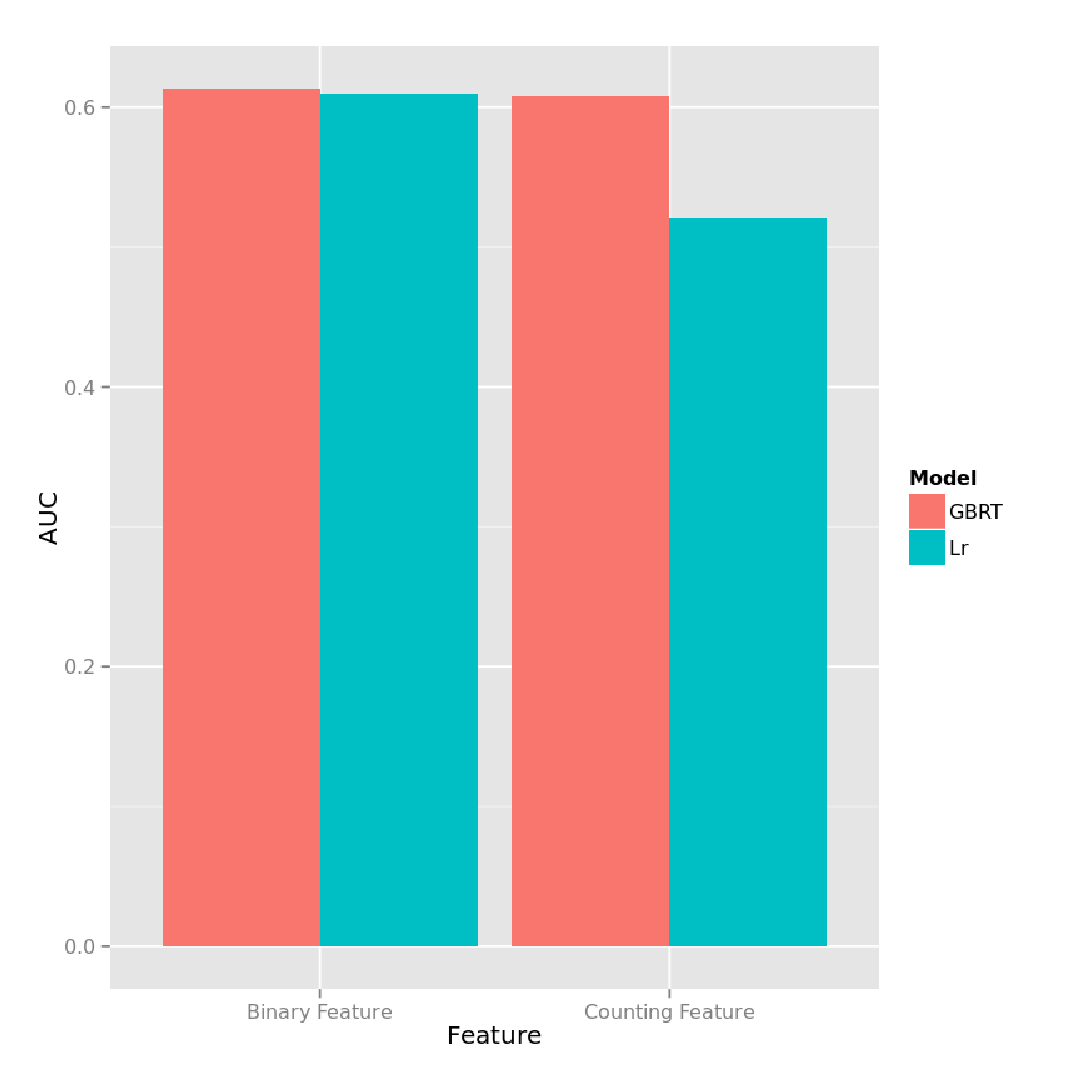
\includegraphics[width=\columnwidth]{2261.eps}
%\caption{Performance 2261}
%\label{fig:2261}
%\end{figure}

%\begin{figure}[t]
%\centering
%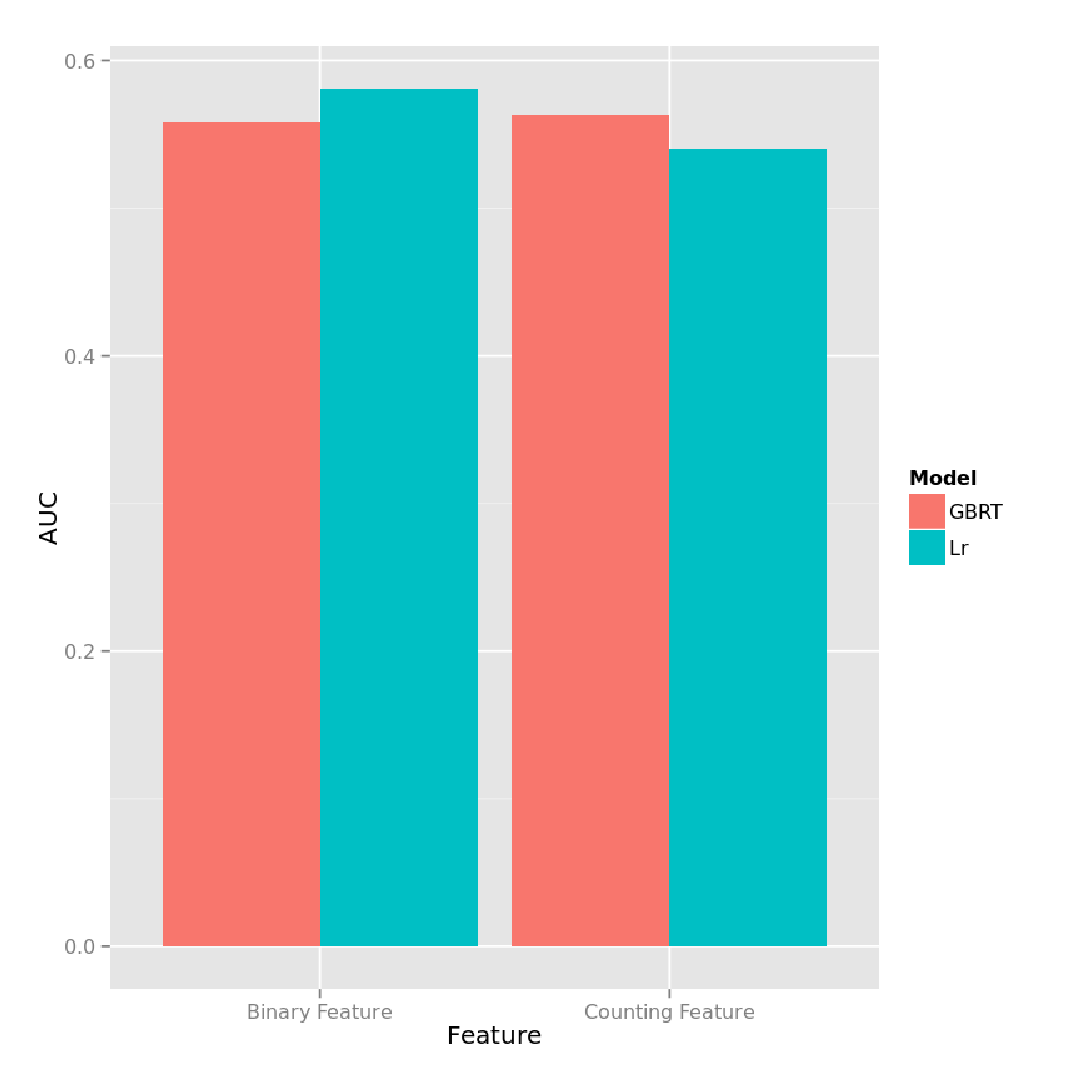
\includegraphics[width=\columnwidth]{2997.eps}
%\caption{Performance 2997}
%\label{fig:2997}
%\end{figure}

%\begin{figure}[t]
%\centering
%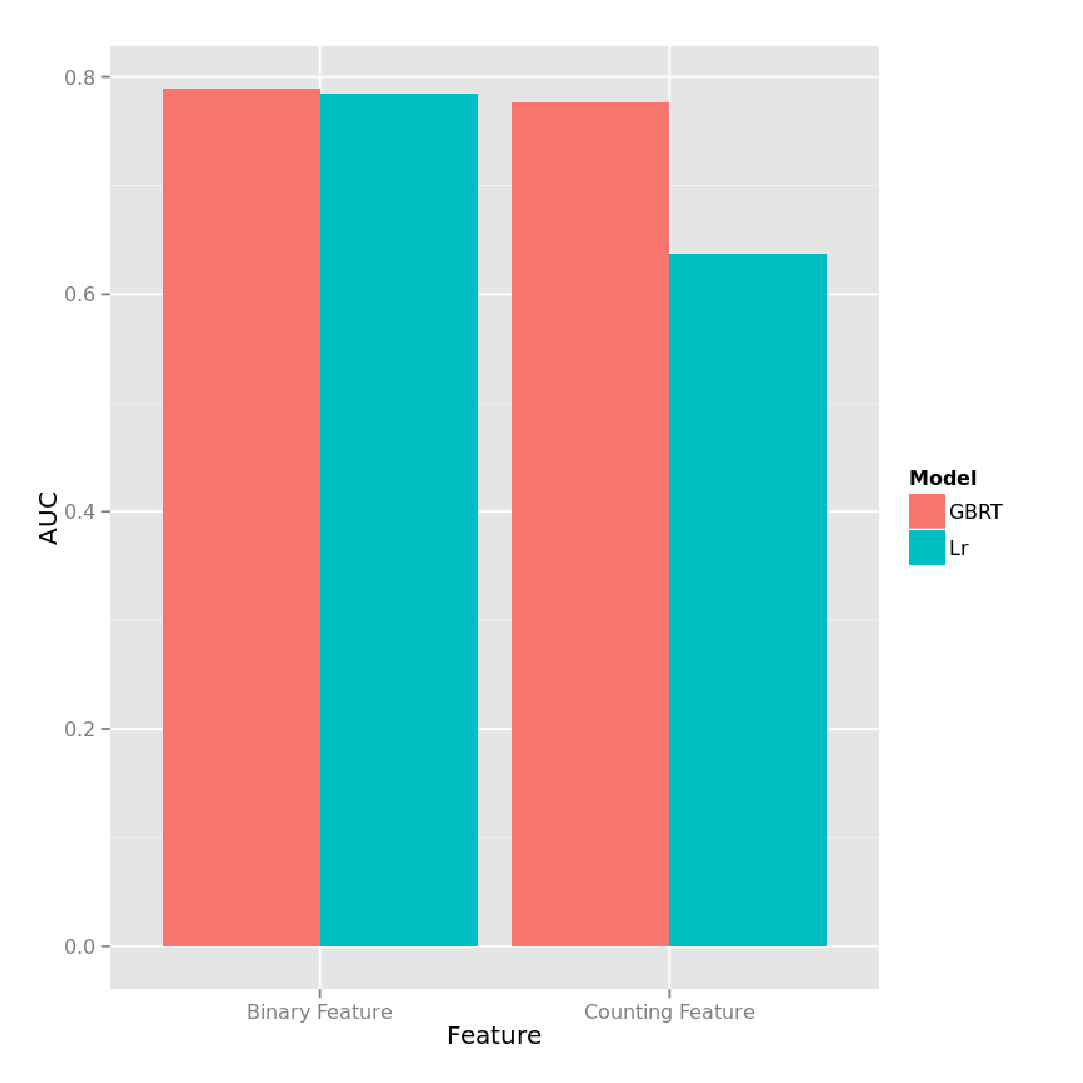
\includegraphics[width=\columnwidth]{3386.eps}
%\caption{Performance 3386}
%\label{fig:3386}
%\end{figure}


% The data from 3-14 to 3-27 are regarded as training dataset, the data from 5- are regarded as test dataset, the count of training dataset is, test dataset is ~\ref{tab:campainid}

% \begin{table*}[h]
% \centering
% \begin{tabular}{ |c|c|c|c| } 
% \hline
% Shared Campaign  & Unique Train Dataset Campaign & Unique Test Dataset Campaign \\
% \hline
% 1310190 & 1307617, 884194, 1283235, 1335301  & 1466432, 1448738 \\ 
% & 1385319, 1349577, 1276074, 1363723 & 1406405, 1424966 \\ 
% &  1357245, 1341802, 1341937, 1307838 & 1424330, 1445998 \\ 
% &  1285558, 1358167, 1305663, 1299899 & 1458704, 1454382 \\
% &  1363711, 1386205, 1368830, 1366271 &  1472727, 1452138 \\
% \hline
% \end{tabular}
% \label{tab:campainid}
% \end{table}

% Only the instances from the campaign with more than 500 clicks and 50000 impressions will be remained, the campaigns can be classified as the ones shared by the training and test dataset, the ones unique to training dataset and the one unique to test dataset.  

% \(1/3\) of the training dataset is used as train dataset, \(2/3\) will be used as count dataset. In order to increase the generalization of training dataset to improve the universality of the trained prediction model, four campaign will constitute one training dataset and two campaigns are used to make up a test dataset to decrease the bias of test dataset.  

% For the sake of convenience, the training dataset will be labeled as 1,2,3,4 and 5, from top to the bottom, as well as the test dataset. For each training dataset, the prediction model will be build based on it which will be used to test the data stream from each of the test dataset, the result is in 6.3.





%Figure \ref{fig:variance} shows that the variance and mean for binary and counting feature dataset are nearly the same. 

%figure \ref{fig:three graphs} shows that the similarity among weights space for counting feature is higher than counting feature. 



\iffalse
Experiment 1.1: Training Dataset  (20762), Test Dataset  (15140) in Figure~\ref{fig:fig1}.:
\begin{figure}[h]
\centering
\includegraphics[width=\columnwidth]{20762_15140.eps}
\caption{Training Dataset  (20762), Test Dataset  (15140)}
\label{fig:fig1}
\end{figure}

Experiment 1.2: Training Dataset  (20762), Test Dataset  (1371) in Figure~\ref{fig:fig2}.:
\begin{figure}[h]
\centering
\includegraphics[width=\columnwidth]{20762_1371.eps}
\caption{Training Dataset  (20762), Test Dataset  (1371)}
\label{fig:fig2}
\end{figure}

Experiment 1.3: Training Dataset  (20762), Test Dataset  (12482) in Figure~\ref{fig:fig2}.:
\begin{figure}[h]
\centering
\includegraphics[width=\columnwidth]{20762_12482.eps}
\caption{ Training Dataset  (20762), Test Dataset  (12482)}
\label{fig:fig2}
\end{figure}

Experiment 2.1: Training Dataset  (15140), Test Dataset  (20762) in Figure~\ref{fig:fig3}.:
\begin{figure}[h]
\centering
\includegraphics[width=\columnwidth]{15140_20762.eps}
\caption{Training Dataset  (15140), Test Dataset  (20762)}
\label{fig:fig3}
\end{figure}

Experiment 2.2: Training Dataset  (15140), Test Dataset  (1371) in Figure~\ref{fig:fig4}.:
\begin{figure}[h]
\centering
\includegraphics[width=\columnwidth]{15140_1371.eps}
\caption{Training Dataset  (15140), Test Dataset  (1371)}
\label{fig:fig4}
\end{figure}

Experiment 2.3: Training Dataset  (15140), Test Dataset  (12482) in Figure~\ref{fig:fig5}.:
\begin{figure}[h]
\centering
\includegraphics[width=\columnwidth]{15140_12482.eps}
\caption{Training Dataset  (15140), Test Dataset  (12482) }
\label{fig:fig5}
\end{figure}

Experiment 3.1: Training Dataset  (1371), Test Dataset  (20762) in Figure~\ref{fig:fig6}.:
\begin{figure}[h]
\centering
\includegraphics[width=\columnwidth]{1371_20762.eps}
\caption{ Training Dataset  (1371), Test Dataset  (20762)}
\label{fig:fig6}
\end{figure}

Experiment 3.2: Training Dataset  (1371), Test Dataset  (15140) in Figure~\ref{fig:fig7}.:
\begin{figure}[h]
\centering
\includegraphics[width=\columnwidth]{1371_15140.eps}
\caption{Training Dataset  (1371), Test Dataset  (15140)}
\label{fig:fig7}
\end{figure}

Experiment 3.3: Training Dataset  (1371), Test Dataset  (12482) in Figure~\ref{fig:fig8}.:
\begin{figure}[h]
\centering
\includegraphics[width=\columnwidth]{1371_12482.eps}
\caption{Training Dataset  (1371), Test Dataset  (12482)}
\label{fig:fig8}
\end{figure}

Experiment 4.1: Training Dataset  (12482), Test Dataset  (20762) in Figure~\ref{fig:fig9}.:
\begin{figure}[h]
\centering
\includegraphics[width=\columnwidth]{12482_20762.eps}
\caption{Training Dataset  (12482), Test Dataset  (20762)}
\label{fig:fig9}
\end{figure}

Experiment 4.2: Training Dataset  (12482), Test Dataset  (1371) in Figure~\ref{fig:fig10}.:
\begin{figure}[h]
\centering
\includegraphics[width=\columnwidth]{12482_1371.eps}
\caption{Training Dataset  (12482), Test Dataset  (1371)}
\label{fig:fig10}
\end{figure}

Experiment 4.2: Training Dataset  (12482), Test Dataset  (15140) in Figure~\ref{fig:fig11}.:
\begin{figure}[h]
\centering
\includegraphics[width=\columnwidth]{12482_15140.eps}
\caption{Training Dataset  (12482), Test Dataset  (15140)}
\label{fig:fig11}
\end{figure}

\fi


